\chapter{Static Analysis}
\label{chap:StaticAnalysis}

In \myBookName{Secure Programming with Static Analysis} \textbf{static analysis} is defined as followed:

\begin{quotation}
``The term static analysis refers to any process for assessing code without
executing it. Static analysis is powerful because it allows for the quick consideration of many possibilities. A static analysis tool can explore a large number of 'what if' scenarios without having to go through all the computations
necessary to execute the code for all the scenarios.''\footnote{\citep[3]{SecureProgramming}}
\end{quotation}

Another definition that highlights the use of prediction during the process of analysis can be found in \myBookName{Principles of program analysis}:

\begin{quotation}
``Program analysis offers static compile-time techniques for predicting safe and computable approximations to the set of values or behaviours arising dynamically at run-time when executing a program on a computer.''\footnote{\citep[1]{ProgramAnalysis}}
\end{quotation}

Thus, tools performing static analysis evaluate software in the abstract, without running the software or considering a specific input.\footnote{\citep[1]{UsingSAToFindBugs}}

Complementary to static program analysis, there is \textbf{dynamic program analysis}, which analyses software at run-time. Unit testing comes to mind as a prominent example of dynamic program analysis.

\newpage
\section{Area of Application}
\label{sec:AreaOfApplication}

The general purpose of static analysis is to extract useful information from source code or compiled code (like byte code or binary code).

The type of information retrieved depends on the context and purpose of the static analysis and can be broken down into the following categories:

\begin{itemize}\addtolength{\itemsep}{-0.5\baselineskip}
\item Program correctness
\item Software security
\item Style checking
\item Program understanding
\item Optimization
\end{itemize}

\subsection{Program Correctness}

Static analysis tools that are concerned with program correctness try to detect defects at compile-time so that these defects do not manifest in run-time errors, such as crashes, data corruption and program malfunctioning. Thus these tools, which are mostly concerned with \textbf{software quality}, are often referred to as \textbf{bug finders}.

Bug finders point out places in the source code, where the program will behave in a way that the programmer did not intend. Most tools are easy to use because they come pre-stocked with a set of \mySlang{bug idioms} (rules) that describe patterns in code that often indicate bugs.\footnote{\citep[32]{SecureProgramming}} They help to find these often hard-to-spot defects early in the software development life-cycle, reducing the cost, time, and risk of software errors.\footnote{\citep{CovertySA}}

A prominent example of preventing run-time errors at compile-time is type checking. In this sense, compilers themselves can be seen as static analysis tools and - as we will see later - both have much in common.

\begin{quotation}
``The lint program for C programs is generally considered the first widely used static analysis tool for defect detection.''\footnote{\citep[1]{UsingSAToFindBugs}}
\end{quotation}

\subsubsection{Generic and Context-Specific Defects}

Defects can be categorized into generic and context-specific defects.

\textbf{Generic defects} are problems that can occur in almost any program written in the given programming language, such as buffer overflows and memory leaks.\\
\textbf{Context-specific defects} on the other hand require specific knowledge about the semantics of the given program.\footnote{\citep[14]{SecureProgramming}} Applications that deal with atomic operations (like a program that handles money transfer) belong to the latter category.

The following sections will present different kinds of bugs, most of which can be found by analysing the control and data flow of an application.

\subsubsection{Overflow and Range Analysis Problems}

A buffer overflow occurs when a program writes data outside the bounds of allocated memory\footnote{\citep[175]{SecureProgramming}}, for example when writing data into a buffer that is too small for the data to be written, leading to the memory after the buffer being overwritten and thus corrupted. Static analysis tools can detect such problems and advice the programmer to do a bounds-check.

An integer overflow occurs when an integral value is increased or decreased beyond its capacity\footnote{\citep[235]{SecureProgramming}}. The following example demonstrates how this can lead to an infinite loop:

\SingleSpacing
\begin{lstlisting}[language=C++, caption=Integer \mySlang{underflow} in \myProperName{C++}]
for(unsigned int i = 200; i >= 0; --i)
{
	// ...
}
\end{lstlisting}
\OnehalfSpacing

A static analysis tool will detect that the expression \mySCName{i \textgreater= 0} will always be true for \mySCName{unsigned} integer types like \mySCName{i}, as \mySCName{i} will be set to the highest possible unsigned integer when being \mySCName{0} and decreased by \mySCName{1}.

\subsubsection{Resource Leaks}

Resource leaks can be detected by tracking request (for example allocation of memory) and release of resources.

If a program gives up all references to a resource that has not been released, the resource is leaked. On the other hand, using a resource that has not been requested properly or releasing an already released resource may lead to unexpected results or even crashes.

The most prominent example of a resource leak is a memory leak. But there are other important resources like files and databases that may need to be locked before usage and released afterwards.

\subsubsection{Threads and Concurrency}

Static analysis tools can also be used to find problems with threads such as data races and deadlocks.

Similar to the detection of resource leaks, the data and call flow of the application can be analysed to track the locking and unlocking of semaphores.

\subsubsection{Other Problems and Warnings}

There are many more possible sources for bugs that can be detected using static analysis tools, such as division by zero, dereferencing of \mySCName{null}-pointers or the returning of references or pointers to local function variables.

Bug finders are not only concerned with finding malicious code that will lead to run-time errors, but may also warn about code that is redundant, like comparisons that will always have the same result. Although such a comparison will not cause a failure or exception, its existence suggests that it might have resulted from a coding error, leading to incorrect program behaviour.\footnote{\citep[1]{UsingSAToFindBugs}}

Similar warnings could be issued for functions whose return values (for example error codes) have not been checked or for exception catch-clauses that are too broad, so that they catch important exceptions like \mySCName{OutOfMemoryError} without handling them.

\subsection{Software Security}

\begin{quotation}
``Static analysis is particularly well suited to security because many security problems occur in corner cases and hard-to-reach states that can be difficult to exercise by actually running the code.''\footnote{\citep[4]{SecureProgramming}}
\end{quotation}

Concerning software security, static analysis tools are used to find coding errors before they can be exploited. Buffer overflows and format string vulnerabilities come to mind, possibly resulting in \myProperName{SQL} injection, cross-site scripting or unwarranted acquisition of administrator privileges. 

Static analysis may also track input data flow and validation to determine
all the implicit ways a program might be putting unwarranted faith in some aspect of its input.\footnote{\citep[172]{SecureProgramming}}

\subsection{Style Checking}

Style checkers enforce rules related to whitespace, position of scope-brackets, naming conventions, deprecated functions, commenting, program structure, and similar non-semantic issues.\footnote{\citep[25]{SecureProgramming}}

\subsection{Program Understanding}

\begin{wrapfigure}{r}{0.4\textwidth}
  \vspace{-20pt}
  \begin{center}
    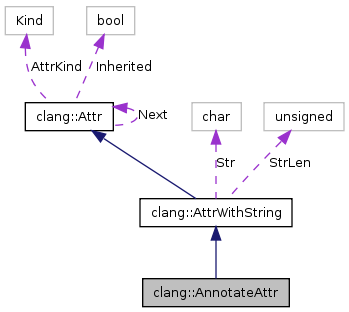
\includegraphics[scale=0.5]{Images/ClangGraph.png}
  \end{center}
  \caption{\myProperName{Doxygen} output of class relationships in \myProperName{Clang}}
  \label{fig:ClangGraph}
   \vspace{-15pt}
\end{wrapfigure}

Program understanding tools help users make sense of large codebases.\footnote{\citep[27]{SecureProgramming}} Most modern IDE's provide functionality for helping the user navigate the codebase, for example jumping to a function's definition or finding all uses of a method. Some even provide functionality for refactoring symbols, like renaming classes. All these operations need knowledge about the symbols existing in the codebase.

Other tools visualize the source code, for example by creating \myProperName{UML} diagrams from source, rendering images of class hierarchies or function callgraphs that can help the user understand the control flow of the application and the relationships between the existing symbols.

Prominent tools like \myProperName{Doxygen}\footnote{\myProperName{Doxygen}: \url{http://www.stack.nl/~dimitri/doxygen/}} automatically create documentation from source code and code comments.

\subsection{Optimization}

Compilers use static analysis to perform code optimization:

\begin{quotation}
``A main application is to allow compilers to generate code avoiding redundant computations, e.g. by reusing available results or by moving loop invariant computations out of loops, or avoiding superfluous computations, e.g. of results known to be not needed or of results known already at compile-time.''\footnote{\citep[1]{ProgramAnalysis}}
\end{quotation}

Apart from code optimization, compile-time optimization, for example by finding \linebreak unnecessary include-files in \myProperName{C++} applications is another area that static analysis is used for. \myProperName{include-what-you-use}\footnote{\myProperName{include-what-you-use}: \url{http://code.google.com/p/include-what-you-use/}} is a tool that performs this task. It internally uses the \myProperName{Clang} compiler.

\section{Static Analysis as Part of a Programmer's Workflow}

Being major factors of software quality, companies put a lot of effort into improving and verifying \textbf{program correctness} and \textbf{software security}. Different techniques have been developed, each concerned with achieving this main goal, but taking varying routes and targeting different stages of the development.

\textbf{Software engineering} and planning begin long before any program code is written, specifying program behaviour and design, and finding structural problems and security concerns before implementation. \textbf{Pair programming} aims at reducing coding errors and making design choices at the time of writing program code by using human experience and communication. \textbf{Code review} is similar, but happens at a later stage. \textbf{Dynamic testing}, including unit tests, has been invented to verify correct run-time program behaviour of written code programmatically, with the help of more program code that tests implementations and compares the results to the expected output.

All these techniques follow a defensive mindset about developing applications, knowing that every programmer, no matter how experienced, will make mistakes that lead to undefined program behaviour. All in all these techniques aim at reducing the rate of errors that go unnoticed.

\textbf{Static analysis} is another technique in the programmer's toolbox serving this goal, during and after code creation. Compared to dynamic testing and code review, it reduces the human factor, programatically applying \myInlineQuote{checks thoroughly and consistently, without any of the bias that a programmer might have about which pieces of code are 'interesting' (...) or which pieces of code are easy to exercise through dynamic testing.}\footnote{\citep[22]{SecureProgramming}} Static analysis tools accumulate the knowledge of experienced programmers and as \myAuthorName{Brian Chess} and \myAuthorName{Jacob West} point out, the feedback given by these tools acts as a means of knowledge transfer by showing the programmer types of errors he was not aware of.\footnote{\citep[22]{SecureProgramming}} In this way, a \myInlineQuote{static analysis tool can make the code review process faster and more fruitful by hypothesizing a set of potential problems for consideration during a code review.}\footnote{\citep[13]{SecureProgramming}}

As with dynamic testing and code review, static analysis can not verify the absence of errors, but is a technique to reduce the amount of bugs before release.

\subsection{Drawbacks}

As every technique, static analysis has drawbacks. 

Depending on how well a tool works and how good it is balanced, static analysis tools may produce a lot of \textbf{false positives}, meaning pointing out an error where none exists. Too much \mySlang{noise} is problematic, as it costs the programmer valuable time to check if a result is really a bug or not. Also, real problems may be overseen, when false positives dominate the tools output.

\textbf{False negatives}, on the other hand, are real bugs that a tool did not discover. It has already been said, that complete absence of errors can not be proven with any tool - so, using static analysis tools may give the programmer a false sense of security.\footnote{\citep[23]{SecureProgramming}}


\section{Static Analysis Tool Internals}

To retrieve useful information from the code, static analysis tools need to build an internal representation (model) of the program to be analysed. The structure of that model heavily depends on the purpose of the tool and has to make good trade-offs between precision, depth, and scalability.\footnote{\citep[45]{SecureProgramming}} After such a model has been created, the tool can use the information for further processing. It could, for example, perform rule-based checks on the model to find coding errors.

\subsection{The Model}

When creating the internal program model, static analysis tools generally borrow a lot from the compiler world\footnote{\citep[72]{SecureProgramming}}. They especially follow the first two phases of a compiler: lexical analysis and syntax analysis.

\begin{quotation}
``\textbf{Lexical analysis} (...) is the initial part of reading and analysing the program text: The text is read and divided into \textit{tokens}, each of which corresponds to a symbol in the programming language, e.g., a variable name, keyword or number.''\footnote{\citep[2]{CompilerBasics}}
\end{quotation}

Compared to compilers, static analysis tools may filter out less during lexical analysis. They may preserve comments, in case the tool needs information from comments for the model (\myProperName{Doxygen} is a prominent example for this case).
Static analysis tools that search for coding errors usually also associate the tokens with their source code positions for later error reporting.\footnote{\citep[72]{SecureProgramming}} 

\begin{quotation}
``\textbf{Syntax analysis} (...) takes the list of tokens produced by the lexical analysis and arranges these in a tree-structure (called the \textit{syntax tree}) that reflects the structure of the program. This phase is often called \textit{parsing}.''\footnote{\citep[2]{CompilerBasics}}
\end{quotation}

As the created syntax tree contains a lot of irrelevant data that is not needed for later analysis (parentheses, etc.), the syntax tree is usually transformed into an \textbf{abstract syntax tree (AST)}, where such information is either removed or combined from multiple tree nodes into single ones.\footnote{\citep[99]{CompilerBasics}}

Some static analysis tools may go their own way from this point on and create their model based on the abstract syntax tree.\\Other tools, like bug finders, as well as compilers for statically typed languages will perform another phase common in the compiler world: \textbf{semantic analysis}. During that phase, a symbol table will be build, which associates each identifier found in the program with its type and a pointer to its declaration or definition.\footnote{\citep[76]{SecureProgramming}} Using the created table, the tool or compiler is able to perform type checking to check the correctness of the program.\footnote{\citep[76]{SecureProgramming}}

Bug finders additionally need to populate their model with information about the effects of library or system calls invoked by the program being analysed.\footnote{\citep[37]{SecureProgramming}}

\subsection{Applying Rules}

After creating a model, static analysis tools that check for correctness, will perform checks on the model using a set of rules that are delivered with the tool. These rules may search for common \mySlang{bug idioms} like memory leaks, buffer overflows or may define the characteristics of a special security related problem.

Some tools allow the user to extend the set of rules to search for bugs that may be specific to the user's codebase or that are not found by the rules delivered with the tool.\footnote{\citep[97]{SecureProgramming}}

For altering the output of the static analysis tool, some bug finders allow the annotation of source code passages.\footnote{\citep[99]{SecureProgramming}} An annotation can be helpful to suppress a false positive in the output.
\\For languages that do not provide special syntax for annotations, as \myProperName{Java} and \myProperName{C\#} do, annotations usually
take the form of specially formatted comments.\footnote{\citep[99]{SecureProgramming}}

The approaches that are used for checking rules differ from rule to rule. Some checks track control flow or data flow throughout the program. Others use alternative relationships that can be drawn from the model. How static analysis tools perform these checks is out of the scope of this thesis. For further knowledge the reader is advised to gather information about \textit{Control Flow Analysis}, \textit{Data Flow Analysis}, \textit{Constraint Based Analysis}, \textit{Taint Propagation}, \textit{Abstract Interpretation}, \textit{Interprocdural Analysis }as well as \textit{Type and Effect Systems}. 

\section{Existing Static Analysis Tools}

The application to be developed will make use of a 3rd party library for performing an integral part of the analysis of \myProperName{C++} headers. 

The most important factor of the chosen static analysis tool/library is its ability to parse \myProperName{C++} and to export or give access to a (simplified) abstract syntax tree of the parsed source files, including symbol and type information. Information about namespaces, global variables, functions including parameters and return types, classes, class-members and more needs to be extracted.

Also, as this project is meant to be open-source, its dependencies must be released in an according licence, which excludes all commercial static analysis tools like \myProperName{Coverty}\footnote{\myProperName{Coverty}: \url{http://www.coverity.com/}}, \myProperName{PVS-Studio}\footnote{\myProperName{PVS-Studio}: \url{http://www.viva64.com/en/pvs-studio/}} or \myProperName{pc-lint}\footnote{\myProperName{pc-lint}: \url{http://www.gimpel.com/html/pcl.htm}}. It is also not known, whether these tools would provide the ability to export symbol and type information.

Further, the chosen library needed to be in active development to adjust to changes coming in the new \myProperName{C++} standard. This excluded a couple of small open source projects that dealt with parsing \myProperName{C++} headers.

The choice had to be made between three projects: \myProperName{GCC-XML}, \myProperName{Dehydra} and \myProperName{Clang}.

\subsection{\myProperName{GCC-XML}}

\myProperName{GCC-XML}\footnote{\myProperName{GCC-XML}: \url{http://www.gccxml.org/HTML/Index.html}} is an extension to \myProperName{GCC}'s \myProperName{C++} parser that outputs AST information into an \myProperName{XML} file. It does not seem to provide any means of filtering the output. The developed application would need to parse the \myProperName{XML} and build its own representation internally. Hence, \myProperName{GCC-XML} only gives indirect access to \myProperName{GCC}'s syntax tree and is thus not well-suited for solving the problem.

\subsection{Dehydra}

\begin{quotation}
``Dehydra is a lightweight, scriptable, general purpose static analysis tool capable of application-specific analyses of C++ code (...) [that] is built as a GCC plugin, (...).''\footnote{\citep{MDNDehydra}}
\end{quotation}

\myProperName{Dehydra}\footnote{\myProperName{Dehydra}: \url{https://developer.mozilla.org/en/Dehydra}} is developed by \myProperName{Mozilla} for checking specific bug patterns in its large codebase for \myProperName{Firefox} and other \myProperName{Mozilla} applications. It allows custom querying of the AST with the help of \myProperName{JavaScript} scripts.

When compiling a project with \myProperName{GCC} and \myProperName{Dehydra}, the user provides a script file along with the command-line arguments. As the compilation happens, functions in the given script are called to inform about found types, functions and other symbols. This way the script can build its own AST representation, filtering symbols on the fly when necessary.

An example function that a script may provide is \mySCName{process\_type(t)}, which is called by \myProperName{Dehydra} whenever a new type was found in the compiling code.

The biggest drawback of \myProperName{Dehydra} is that it is currently only supported on \myProperName{Linux} based operating systems.

\myProperName{Dehydra} was used for implementing \myProperName{DXR}\footnote{\myProperName{DXR}: \url{https://github.com/mozilla/dxr}}, \myProperName{Mozilla}'s web source code cross-reference tool, that can be used to navigate inside the \myProperName{Mozilla} code base. \myProperName{DXR} development moved to using \myProperName{Clang} in newer builds, though.

\subsection{\myProperName{Clang} and \myProperName{libclang}}
\label{sec:Clang}

\begin{quotation}
``Clang is an 'LLVM native' C/C++/Objective-C compiler, which aims to deliver amazingly fast compiles (...), extremely useful error and warning messages and to provide a platform for building great source level tools. The Clang Static Analyzer is a tool that automatically finds bugs in your code, and is a great example of the sort of tool that can be built using the Clang frontend as a library to parse C/C++ code.''\footnote{\citep{LLVMHP}}
\end{quotation}

\myInlineQuote{The LLVM Project is a collection of modular and reusable compiler and toolchain technologies}. The \myProperName{LLVM} compiler framework includes multiple compiler front-ends, like \myProperName{Clang} for the \myProperName{C} language family, an optimizer and code generation support for many popular CPUs.\footnote{\citep{LLVMHP}}

The open-source \myProperName{Clang}\footnote{\myProperName{Clang}: \url{http://clang.llvm.org/}} project is not only concerned with developing a compiler that produces high-performance code, but also with developing software that can be used in utilities like IDE's and bug finders to perform source code analysis and indexing.

There are two approaches of how an application can integrate \myProperName{Clang} for analysing purposes.
\\On the one hand, one can include \myProperName{Clang} itself as a library and use the internal structures and functions of the compiler, thus having access to the AST build by \myProperName{Clang} in a direct way.
\\The second approach is to use \myProperNameImp{libclang}, a \myProperName{C}-API to \myProperName{Clang}, which exposes much of \myProperName{Clang}'s functionality for indexing source code and accessing ASTs, while maintaining a stable interface independent of changes internal to \myProperName{Clang}. \myProperName{libclang} is extended on a per-need-basis and may thus not provide all features needed for a static analysis tool that builds upon it. As it is an open-source project, these features can easily be added.

\myProperName{Clang} works on all popular operating systems, including \myProperName{Microsoft Windows}. Having this advantage over \myProperName{Dehydra}, \myProperName{Clang} is the favourite choice for use in this project. A detailed description of how \myProperName{libclang} is used inside the application can be found in \myRefChapter{chap:AnalysingCPP}.

\subsubsection{\myProperName{Emscripten}}

In the context of this thesis, another interesting \myProperName{LLVM}-based project should be mentioned: \myProperName{Emscripten}\footnote{\myProperName{Emscripten}: \url{http://emscripten.org}}. 

\begin{quotation}
``Emscripten is an LLVM-to-JavaScript compiler. It takes LLVM bitcode (which can be generated from C/C++ using Clang, or any other language that can be converted into LLVM bitcode) and compiles that into JavaScript, which can be run on the web.''\footnote{\citep{EmscriptenHP} - taken from front page}
\end{quotation}

Instead of accessing \myProperName{C++} through glue code, the \myProperName{C++} code itself is completely compiled to \myProperName{JavaScript}. This may sound very slow in the first place, but with the current performance of \myProperName{JavaScript} virtual machines and the reduced cost of type-conversion (as all is \myProperName{JavaScript}), code generated by \myProperName{Emscripten} is only 3 to 4 times slower than native code generated with \myProperName{GCC}.\footnote{\citep{EmscriptenHP} - taken from FAQ section}